\subsection{Dataset Creation}

Datasets were created to test the performance of the observability model, and to evaluate the performance and impact of the VBEE library on SLAM systems. The datasets were created using a combination of synthetic and real-world data, with the goal of providing a diverse set of scenarios for testing.

\subsection{Observability Scenario Dataset}
\label{sec:observability_scenario_dataset}

The observability scenario dataset is a synthetic set of unique observability scenarios, designed to evaluate the performance of the observability model. The dataset consists of a set of \"worlds\", represented as a spherical volume with a single map point at the center. These worlds contain two types of barriers: keep-out zones, and obstructions. Keep-out zones represent viewpoints relative to the map point that the camera cannot access, like viewpoints that would place the camera below ground. Obstructions on the other hand represent objects that the camera can move behind, but that block the observation of the map point, such as a wall shared with another room. A world consists of the selection of a barrier type for each of the six directions: $x+, y+, z+, x-, y-, z-$. Barriers can be placed either \textit{near} (touching the map point), or \textit{far} (at a distance of $d_{max}/2$ from the map point). Therefore, the choice is made for each direction between the following options:
\begin{itemize}
    \item (0) No obstruction
    \item (1) Near obstruction
    \item (2) Far obstruction
    \item (3) Near keep-out zone
    \item (4) Far keep-out zone
    \item (5) Near obstruction, far keep-out zone
\end{itemize}

A world is defined by a 6-tuple of barrier types $b_{direction}$, representing the selection of barrier type for each of the 6 directions.
\[
    world = (b_{x^+}, b_{y^+}, b_{z^+}, b_{x^-}, b_{y^-}, b_{z^-})
\]
For example, the world $(0, 0, 0, 0, 0, 0)$ would represent a world with no barriers, essentially a map point in free space. The world $(1, 0, 0, 0, 0, 0)$ would represent a world with a near obstruction in the $x^+$ direction, such as a map point that exists on a wall to a shared room. This definition allows for a total of $6^6 = 46,656$ unique worlds, each representing a unique combination of barriers, however, it should be noted that not all combinations are valid, and some combinations are equivalent. Invalid worlds are those that would not allow the map point to be observed from any direction, meaning any world that contains two near barriers in opposing directions. These can be eliminated by removing any worlds where $world[i] \in \{1, 3, 5\} \land world[i+3]\in \{1, 3, 5\} \text{ for } i \in [0, 1, 2]$. Next, any world that is a reflection about any combination of the $x, y, z$ axes can be eliminated, as these worlds are equivalent in terms of observability. Finally, any world that is rotation of another world is eliminated, as these worlds do not provide any additional information. This leaves a total of 896 unique worlds, which are used to evaluate the performance of the observability model.

This dataset allows the observability model to be tested against a wide range of observability scenarios, utilizing the unique worlds as a ground-truth for the observability model's predictions. These worlds can be queried to determine whether a map point is observable from a given viewpoint, and the model can be evaluated based on its ability to predict the observability of the map point from that viewpoint. Figure \ref{fig:world_obs} shows an example of a world with two far obstructions, and a far keep-out zone queried with 1000 random viewpoints. Evaluation of the model can be accomplished by comparing the model's predictions to the ground truth observability of the map point in each world.

\begin{figure}[H]
    \centering
    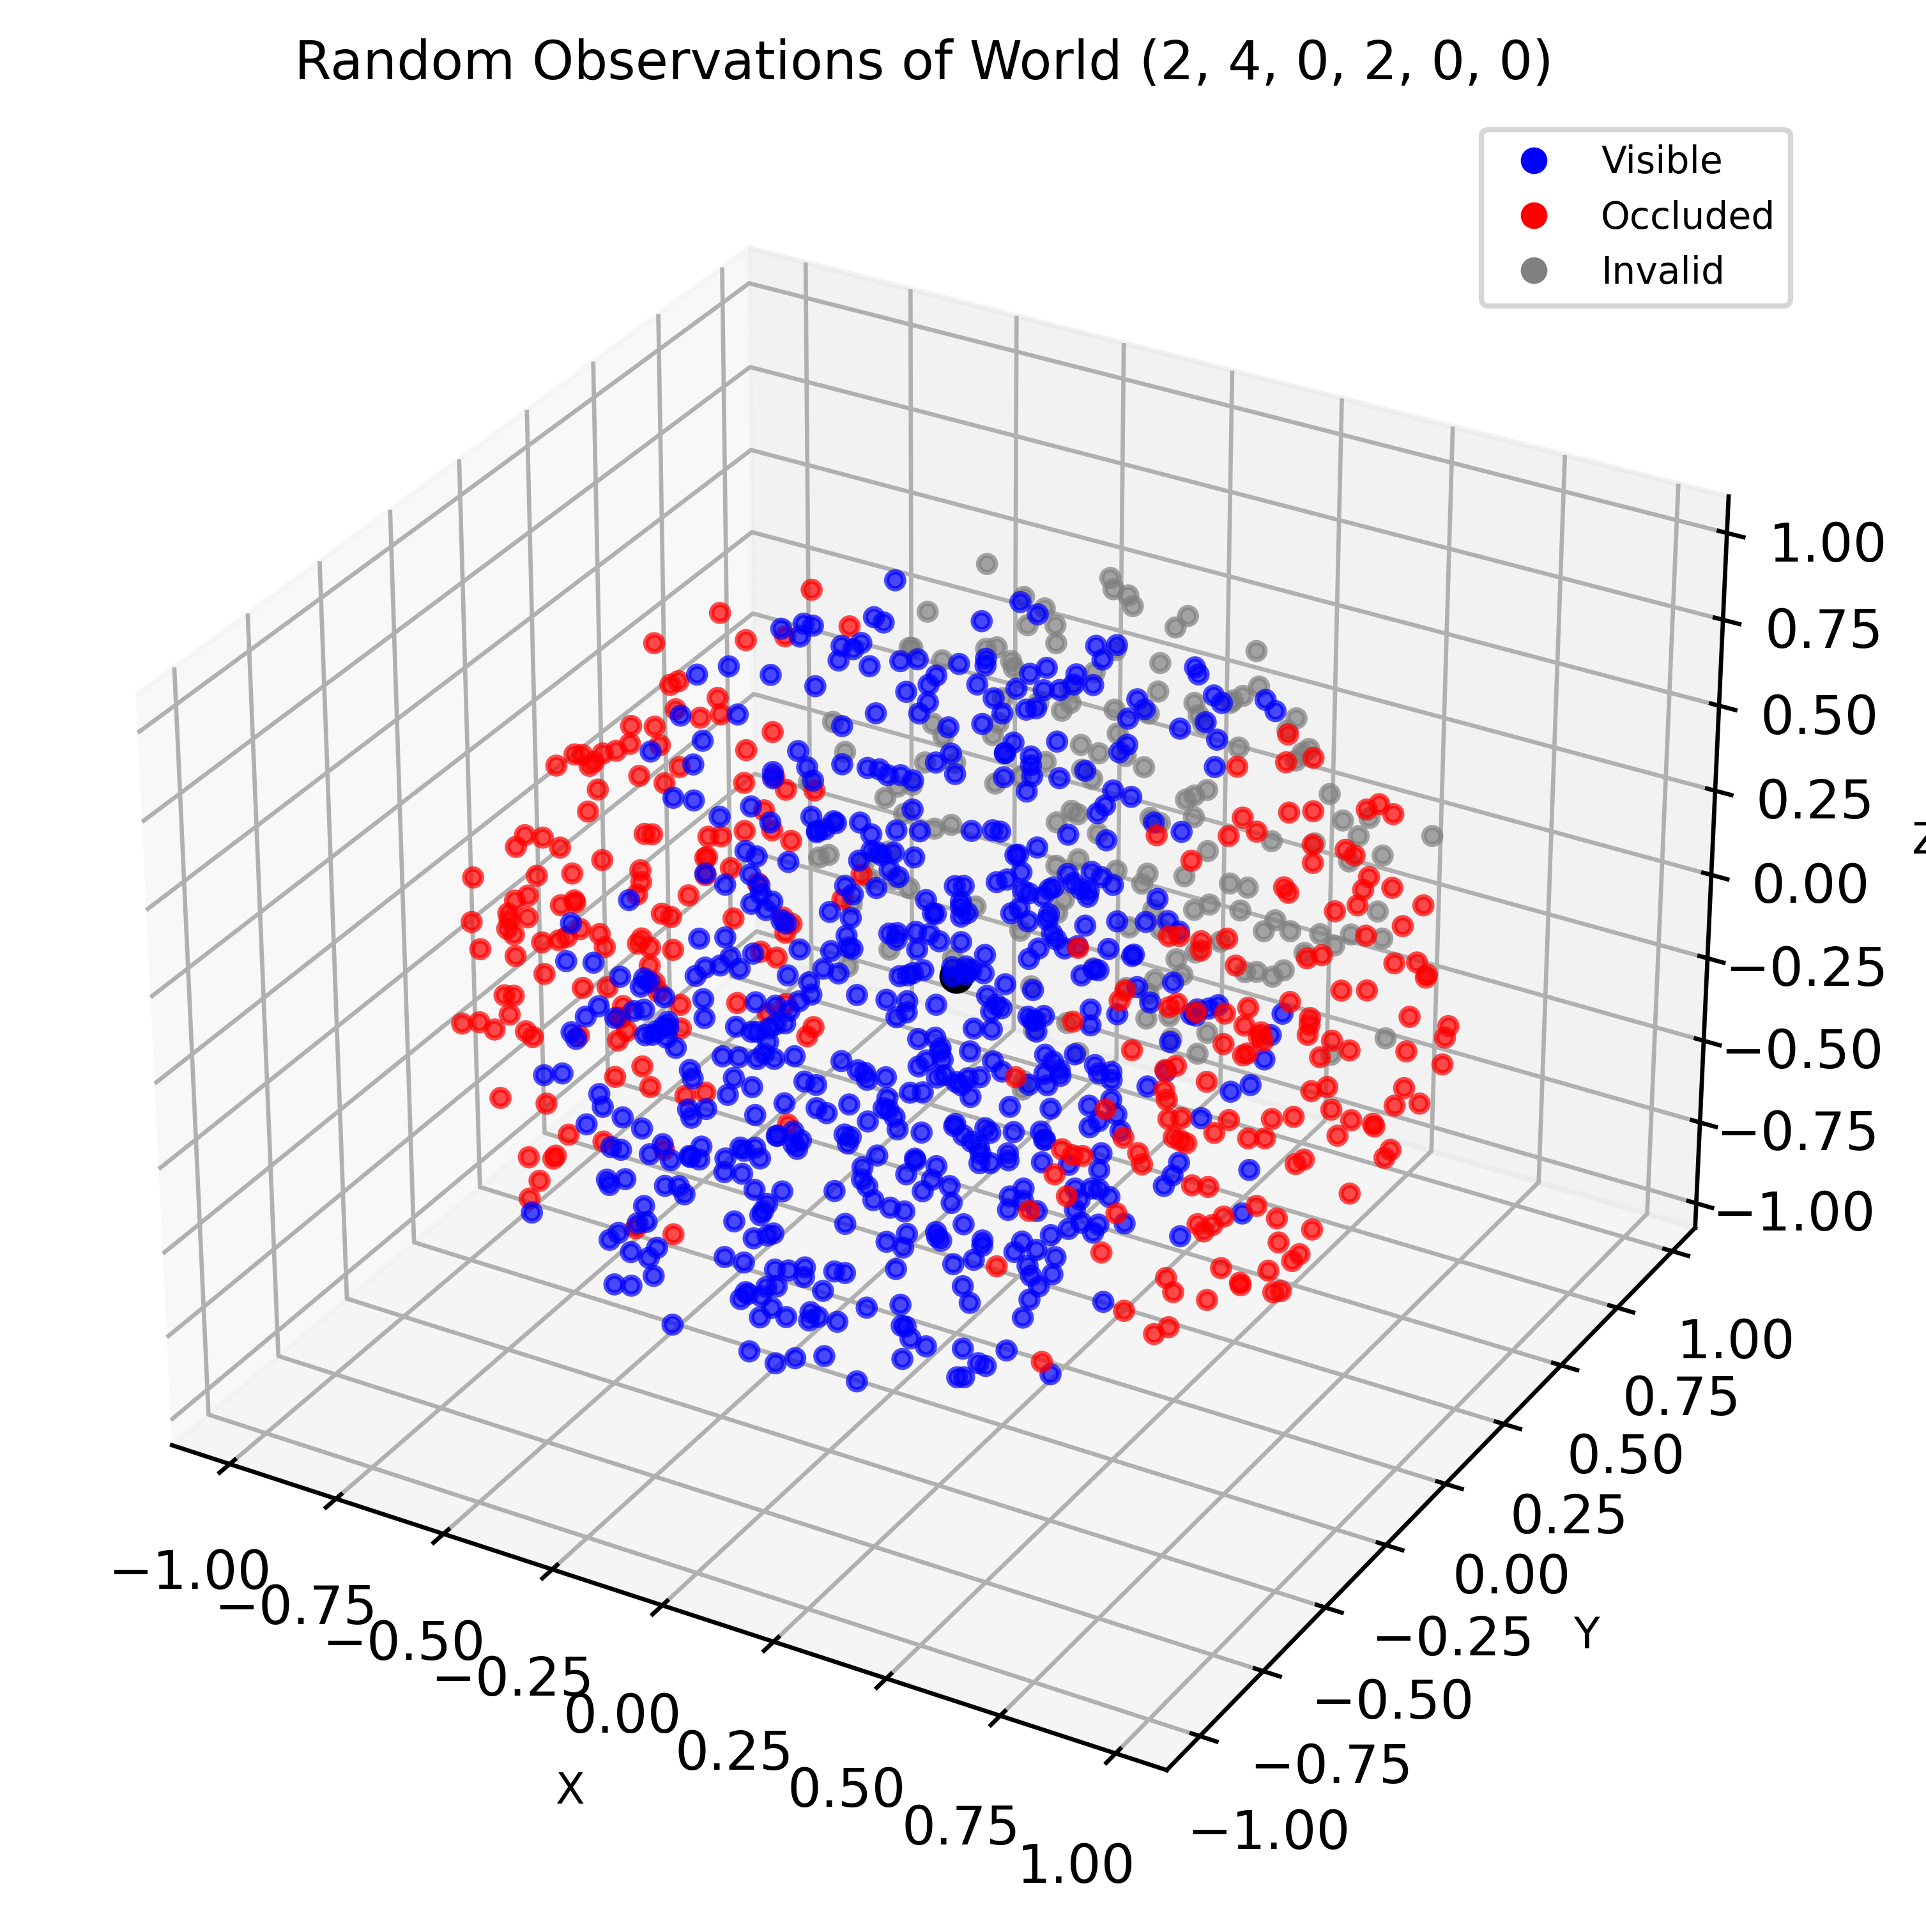
\includegraphics[width=0.8\textwidth]{resources/world_obs.png}
    \caption{1000 random viewpoints of world (2, 4, 0, 2, 0, 0), showing the observability of the map point at the center}
    \label{fig:world_obs}
\end{figure}

\subsubsection{Episodic Visual SLAM Dataset}

To evaluate the performance of the VBEE library in a real-world SLAM system, a stereo visual dataset was created, consisting of a series of trajectories through a household environment. No environmental dynamic changes occur during trajectory recording, but environmental changes do take place between recordings, matching the episodic run modality discussed in Section \ref{sec:background}. Figure \ref{fig:episodic_datasets} shows example images from each trajectory of roughly the same location.

\begin{figure}[H]
    \centering
    
\includegraphics[width=0.8\textwidth]{resources/placeholder.jpeg}
    \caption{Example images from each trajectory of the episodic visual SLAM dataset}
    \label{fig:episodic_datasets}
\end{figure}

This dataset is intended to provide a realistic scenario of episodic visual SLAM operation in a household environment. Ground truth is difficult to obtain in large scale 3D environments, so the dataset is evaluated based on the SLAM system's ability to maintain a consistent map of the environment across multiple trajectories. The VBEE library is integrated into the ORB-SLAM3 system, and the performance of the system is evaluated based on its ability to cull outdated map points and maintain a consistent map across the trajectories.